\documentclass[11pt,preprint]{elsarticle}

\usepackage{lmodern}
%%%% My spacing
\usepackage{setspace}
\setstretch{1.2}
\DeclareMathSizes{12}{14}{10}{10}

% Wrap around which gives all figures included the [H] command, or places it "here". This can be tedious to code in Rmarkdown.
\usepackage{float}
\let\origfigure\figure
\let\endorigfigure\endfigure
\renewenvironment{figure}[1][2] {
    \expandafter\origfigure\expandafter[H]
} {
    \endorigfigure
}

\let\origtable\table
\let\endorigtable\endtable
\renewenvironment{table}[1][2] {
    \expandafter\origtable\expandafter[H]
} {
    \endorigtable
}


\usepackage{ifxetex,ifluatex}
\usepackage{fixltx2e} % provides \textsubscript
\ifnum 0\ifxetex 1\fi\ifluatex 1\fi=0 % if pdftex
  \usepackage[T1]{fontenc}
  \usepackage[utf8]{inputenc}
\else % if luatex or xelatex
  \ifxetex
    \usepackage{mathspec}
    \usepackage{xltxtra,xunicode}
  \else
    \usepackage{fontspec}
  \fi
  \defaultfontfeatures{Mapping=tex-text,Scale=MatchLowercase}
  \newcommand{\euro}{€}
\fi

\usepackage{amssymb, amsmath, amsthm, amsfonts}

\def\bibsection{\section*{References}} %%% Make "References" appear before bibliography


\usepackage[numbers]{natbib}

\usepackage{longtable}
\usepackage[margin=2.3cm,bottom=2cm,top=2.5cm, includefoot]{geometry}
\usepackage{fancyhdr}
\usepackage[bottom, hang, flushmargin]{footmisc}
\usepackage{graphicx}
\numberwithin{equation}{section}
\numberwithin{figure}{section}
\numberwithin{table}{section}
\setlength{\parindent}{0cm}
\setlength{\parskip}{1.3ex plus 0.5ex minus 0.3ex}
\usepackage{textcomp}
\renewcommand{\headrulewidth}{0.2pt}
\renewcommand{\footrulewidth}{0.3pt}

\usepackage{array}
\newcolumntype{x}[1]{>{\centering\arraybackslash\hspace{0pt}}p{#1}}

%%%%  Remove the "preprint submitted to" part. Don't worry about this either, it just looks better without it:
\makeatletter
\def\ps@pprintTitle{%
  \let\@oddhead\@empty
  \let\@evenhead\@empty
  \let\@oddfoot\@empty
  \let\@evenfoot\@oddfoot
}
\makeatother

 \def\tightlist{} % This allows for subbullets!

\usepackage{hyperref}
\hypersetup{breaklinks=true,
            bookmarks=true,
            colorlinks=true,
            citecolor=blue,
            urlcolor=blue,
            linkcolor=blue,
            pdfborder={0 0 0}}


% The following packages allow huxtable to work:
\usepackage{siunitx}
\usepackage{multirow}
\usepackage{hhline}
\usepackage{calc}
\usepackage{tabularx}
\usepackage{booktabs}
\usepackage{caption}


\newenvironment{columns}[1][]{}{}

\newenvironment{column}[1]{\begin{minipage}{#1}\ignorespaces}{%
\end{minipage}
\ifhmode\unskip\fi
\aftergroup\useignorespacesandallpars}

\def\useignorespacesandallpars#1\ignorespaces\fi{%
#1\fi\ignorespacesandallpars}

\makeatletter
\def\ignorespacesandallpars{%
  \@ifnextchar\par
    {\expandafter\ignorespacesandallpars\@gobble}%
    {}%
}
\makeatother


% definitions for citeproc citations
\NewDocumentCommand\citeproctext{}{}
\NewDocumentCommand\citeproc{mm}{%
\href{\#cite.\detokenize{#1}}{#2}\nocite{#1}}

\makeatletter
% allow citations to break across lines
\let\@cite@ofmt\@firstofone
% avoid brackets around text for \cite:
\def\@biblabel#1{}
\def\@cite#1#2{{#1\if@tempswa , #2\fi}}
\makeatother
\newlength{\cslhangindent}
\setlength{\cslhangindent}{1.5em}
\newlength{\csllabelwidth}
\setlength{\csllabelwidth}{3em}
\newenvironment{CSLReferences}[2] % #1 hanging-indent, #2 entry-spacing
{\begin{list}{}{%
	\setlength{\itemindent}{0pt}
	\setlength{\leftmargin}{0pt}
	\setlength{\parsep}{0pt}
	% turn on hanging indent if param 1 is 1
	\ifodd #1
	\setlength{\leftmargin}{\cslhangindent}
	\setlength{\itemindent}{-1\cslhangindent}
	\fi
	% set entry spacing
	\setlength{\itemsep}{#2\baselineskip}}}
{\end{list}}

\usepackage{calc}
\newcommand{\CSLBlock}[1]{\hfill\break\parbox[t]{\linewidth}{\strut\ignorespaces#1\strut}}
\newcommand{\CSLLeftMargin}[1]{\parbox[t]{\csllabelwidth}{\strut#1\strut}}
\newcommand{\CSLRightInline}[1]{\parbox[t]{\linewidth - \csllabelwidth}{\strut#1\strut}}
\newcommand{\CSLIndent}[1]{\hspace{\cslhangindent}#1}


\urlstyle{same}  % don't use monospace font for urls
\setlength{\parindent}{0pt}
\setlength{\parskip}{6pt plus 2pt minus 1pt}
\setlength{\emergencystretch}{3em}  % prevent overfull lines
\setcounter{secnumdepth}{5}

%%% Use protect on footnotes to avoid problems with footnotes in titles
\let\rmarkdownfootnote\footnote%
\def\footnote{\protect\rmarkdownfootnote}
\IfFileExists{upquote.sty}{\usepackage{upquote}}{}

%%% Include extra packages specified by user

%%% Hard setting column skips for reports - this ensures greater consistency and control over the length settings in the document.
%% page layout
%% paragraphs
\setlength{\baselineskip}{12pt plus 0pt minus 0pt}
\setlength{\parskip}{12pt plus 0pt minus 0pt}
\setlength{\parindent}{0pt plus 0pt minus 0pt}
%% floats
\setlength{\floatsep}{12pt plus 0 pt minus 0pt}
\setlength{\textfloatsep}{20pt plus 0pt minus 0pt}
\setlength{\intextsep}{14pt plus 0pt minus 0pt}
\setlength{\dbltextfloatsep}{20pt plus 0pt minus 0pt}
\setlength{\dblfloatsep}{14pt plus 0pt minus 0pt}
%% maths
\setlength{\abovedisplayskip}{12pt plus 0pt minus 0pt}
\setlength{\belowdisplayskip}{12pt plus 0pt minus 0pt}
%% lists
\setlength{\topsep}{10pt plus 0pt minus 0pt}
\setlength{\partopsep}{3pt plus 0pt minus 0pt}
\setlength{\itemsep}{5pt plus 0pt minus 0pt}
\setlength{\labelsep}{8mm plus 0mm minus 0mm}
\setlength{\parsep}{\the\parskip}
\setlength{\listparindent}{\the\parindent}
%% verbatim
\setlength{\fboxsep}{5pt plus 0pt minus 0pt}



\begin{document}



\begin{frontmatter}  %

\title{QUESTION\_4}

% Set to FALSE if wanting to remove title (for submission)




\author[Add1]{Happy Matope}
\ead{your-student-number@sun.ac.za}





\address[Add1]{Stellenbosch University, South Africa}



\vspace{1cm}


\begin{keyword}
\footnotesize{
Portfolio optimisation \sep Minimum variance \sep Ledoit-Wolf shrinkage
\sep Quarterly rebalancing \sep Backtesting \\
\vspace{0.3cm}
}
\footnotesize{
\textit{JEL classification} G11 \sep C61
}
\end{keyword}



\vspace{0.5cm}

\end{frontmatter}

\setcounter{footnote}{0}



%________________________
% Header and Footers
%%%%%%%%%%%%%%%%%%%%%%%%%%%%%%%%%
\pagestyle{fancy}
\chead{}
\rhead{Building a Constrained Global Balanced Index Fund}
\lfoot{}
\rfoot{\footnotesize Page \thepage}
\lhead{}
%\rfoot{\footnotesize Page \thepage } % "e.g. Page 2"
\cfoot{}

%\setlength\headheight{30pt}
%%%%%%%%%%%%%%%%%%%%%%%%%%%%%%%%%
%________________________

\headsep 35pt % So that header does not go over title




\makeatletter
\@ifundefined{pandocbounded}{%
  \newsavebox\pandoc@box
  \newcommand*\pandocbounded[1]{%
    \sbox\pandoc@box{#1}%
    \Gscale@div\@tempa{\textheight}{\dimexpr\ht\pandoc@box+\dp\pandoc@box\relax}%
    \Gscale@div\@tempb{\linewidth}{\wd\pandoc@box}%
    \ifdim\@tempb\p@<\@tempa\p@\let\@tempa\@tempb\fi
    \ifdim\@tempa\p@<\p@\scalebox{\@tempa}{\usebox\pandoc@box}%
    \else\usebox{\pandoc@box}\fi}%
}{}
\makeatother

\section{\texorpdfstring{Introduction
\label{Introduction}}{Introduction }}\label{introduction}

A balanced index fund aims to deliver steady, diversified growth at a
moderate level of risk. Building one is a constrained optimisation
problem: the manager must decide how much to hold in each asset while
respecting the mandate's limits. Here the fund must be long-only,
rebalanced quarterly, and hold at most 35\% in any single asset, 75\% in
equities, 25\% in bonds and credit, 15\% in commodities and 60\%
offshore. Covariance and mean estimates must use at least ten years of
data, and no asset may be held with less than five years of returns.

This report asks two questions:

\begin{enumerate}
\def\labelenumi{\arabic{enumi}.}
\tightlist
\item
  What do optimised portfolios that satisfy every constraint look like,
  and which constraints bind?
\item
  Do they improve on a simple rules-based balanced portfolio out of
  sample?
\end{enumerate}

Two optimisers are used, following the course's portfolio-optimisation
practicals: minimum variance and maximum Sharpe ratio. Both are compared
with a fixed-weight balanced portfolio.

Section \ref{Data} describes the data, Section \ref{Method} the methods,
Section \ref{Results} the results, and Section \ref{Summary} summarises.

\section{\texorpdfstring{Data \label{Data}}{Data }}\label{data}

Table \ref{tab:assets} lists the 15 candidate assets. The paper refers
to a multi-asset file (MAA) that is not in the data folder, so the
universe is built from the files listed in the question:

\begin{itemize}
\tightlist
\item
  \textbf{Global equity:} four non-overlapping MSCI regions (USA,
  Europe, Japan, Emerging Markets). Overlapping aggregates such as MSCI
  World are left out because they would make the covariance matrix
  nearly singular.
\item
  \textbf{Local equity:} the Large and Mid cap indexes, plus two factor
  indexes, Momentum and Value. The Low Volatility index starts only in
  2024, so the five-year rule excludes it.
\item
  \textbf{Local listed property} (J253).
\item
  \textbf{Bonds:} US and Euro 10-year bond proxies built from yields,
  the All Bond Index (ALBI) and inflation-linked bonds (CILI).
\item
  \textbf{Commodities:} the Bloomberg Commodity index and gold. Brent
  crude is excluded because the series is a futures price, not an
  investable total return.
\end{itemize}

\begin{table}[!htbp]
\centering
\caption{Candidate assets (all series end in September 2026)} 
\label{tab:assets}
\begingroup\scriptsize
\begin{tabular}{llllllr}
  \hline
Asset & Description & Class & Region & Source & Start & Years \\ 
  \hline
MSCI\_USA & MSCI USA (USD TR) & Equity & Global & MSCI\_Indexes & Jan 2010 & 16.8 \\ 
  MSCI\_EU & MSCI Europe (USD TR) & Equity & Global & MSCI\_Indexes & Jan 2010 & 16.8 \\ 
  MSCI\_Jap & MSCI Japan (USD TR) & Equity & Global & MSCI\_Indexes & Jan 2010 & 16.8 \\ 
  MSCI\_EM & MSCI Emerging Markets (USD TR) & Equity & Global & MSCI\_Indexes & Jan 2010 & 16.8 \\ 
  SA\_Large & JSE Top 40 / Large caps (J200) & Equity & Local & Index\_Returns\_Daily & Jan 2015 & 11.8 \\ 
  SA\_Mid & JSE Mid caps (J201) & Equity & Local & Index\_Returns\_Daily & Jan 2015 & 11.8 \\ 
  SA\_Momentum & Momentum factor index (STXMOMJ433) & Equity & Local & Index\_Returns\_Daily & Apr 2017 & 9.5 \\ 
  SA\_Value & Value factor index (STXVALJ433) & Equity & Local & Index\_Returns\_Daily & Apr 2018 & 8.5 \\ 
  SA\_Property & Listed property (J253) & Equity & Local & Monthly\_LCL\_Yield\_Indexes & Jan 2010 & 16.8 \\ 
  US\_10Yr & US 10-year bond (proxy from yields) & Bond & Global & Global\_Bond\_Yields & Jan 2010 & 16.8 \\ 
  EURO\_10Yr & Euro 10-year bond (proxy from yields) & Bond & Global & Global\_Bond\_Yields & Jan 2010 & 16.8 \\ 
  ALBI & All Bond Index & Bond & Local & Monthly\_LCL\_Yield\_Indexes & Jan 2010 & 16.8 \\ 
  CILI & Inflation-linked bond index & Bond & Local & Monthly\_LCL\_Yield\_Indexes & Jan 2010 & 16.8 \\ 
  Bcom\_Index & Bloomberg Commodity index & Commodity & Global & Commodities & Jan 2010 & 16.8 \\ 
  Gold & Gold & Commodity & Global & Commodities & Jan 2010 & 16.8 \\ 
   \hline
\end{tabular}
\endgroup
\end{table}

Three data issues matter.

\begin{itemize}
\tightlist
\item
  \textbf{Bond returns.} The bond series are yields, so a total-return
  proxy is built (Section \ref{Method}). Table \ref{tab:bond} shows it
  behaves as expected. For example, the US proxy lost 16.5\% in 2022
  when yields surged and gained 10.6\% in 2020 when they collapsed,
  close to actual US Treasury returns.
\item
  \textbf{Currency.} Global assets are in US dollars and local assets in
  rand. The data folder contains no exchange rate, so returns cannot be
  converted to a single currency. For a South African investor, rand
  weakness would add to global returns and raise their volatility.
\item
  \textbf{Property.} Listed property is classified as equity. It behaves
  like equity (a 63\% maximum drawdown and correlations of 0.5--0.8 with
  equities), and treating it as a yield asset would let it escape the
  equity cap.
\end{itemize}

\begin{table}[!htbp]
\centering
\caption{Bond total-return proxy: calendar-year returns} 
\label{tab:bond}
\begingroup\footnotesize
\begin{tabular}{lrr}
  \hline
Year & EURO\_10Yr & US\_10Yr \\ 
  \hline
2011 & 0.135 & 0.163 \\ 
  2013 & -0.040 & -0.087 \\ 
  2014 & 0.153 & 0.105 \\ 
  2019 & 0.041 & 0.092 \\ 
  2020 & 0.034 & 0.106 \\ 
  2021 & -0.043 & -0.042 \\ 
  2022 & -0.223 & -0.165 \\ 
  2023 & 0.074 & 0.038 \\ 
   \hline
\end{tabular}
\endgroup
\end{table}

Table \ref{tab:desc} and Figure \ref{Figure1} summarise the assets' risk
and return.

\begin{itemize}
\tightlist
\item
  \textbf{Local bonds offered the best return per unit of risk} since
  2010 (ALBI and CILI, both about 1.26).
\item
  \textbf{US equity was the strongest equity market} (14.3\% a year).
\item
  \textbf{Global bonds returned little} (1--2\% a year), and
  \textbf{broad commodities returned almost nothing}.
\end{itemize}

\begin{table}[!htbp]
\centering
\caption{Descriptive statistics of monthly returns (from 2010, or the asset's start date)} 
\label{tab:desc}
\begingroup\scriptsize
\begin{tabular}{lrrrrrr}
  \hline
Asset & Return (ann.) & SD (ann.) & Return / risk & Max drawdown & Skewness & Excess kurtosis \\ 
  \hline
MSCI\_USA & 0.143 & 0.145 & 0.980 & 0.248 & -0.310 & 0.583 \\ 
  MSCI\_EU & 0.075 & 0.169 & 0.443 & 0.285 & -0.197 & 0.491 \\ 
  MSCI\_Jap & 0.084 & 0.142 & 0.590 & 0.291 & -0.346 & 0.687 \\ 
  MSCI\_EM & 0.061 & 0.179 & 0.344 & 0.357 & -0.068 & 0.603 \\ 
  SA\_Large & 0.109 & 0.151 & 0.725 & 0.199 & 0.127 & 0.534 \\ 
  SA\_Mid & 0.073 & 0.159 & 0.458 & 0.356 & -1.301 & 4.872 \\ 
  SA\_Momentum & 0.100 & 0.159 & 0.631 & 0.277 & -0.641 & 1.695 \\ 
  SA\_Value & 0.109 & 0.165 & 0.659 & 0.322 & -0.556 & 2.921 \\ 
  SA\_Property & 0.099 & 0.188 & 0.524 & 0.626 & -1.605 & 10.805 \\ 
  US\_10Yr & 0.019 & 0.072 & 0.260 & 0.268 & 0.082 & 0.019 \\ 
  EURO\_10Yr & 0.011 & 0.067 & 0.158 & 0.276 & -0.126 & 0.453 \\ 
  ALBI & 0.097 & 0.077 & 1.265 & 0.098 & -0.733 & 2.863 \\ 
  CILI & 0.077 & 0.061 & 1.262 & 0.081 & -0.595 & 2.495 \\ 
  Bcom\_Index & 0.001 & 0.148 & 0.007 & 0.653 & -0.295 & 0.733 \\ 
  Gold & 0.083 & 0.165 & 0.502 & 0.419 & 0.044 & 0.059 \\ 
   \hline
\end{tabular}
\endgroup
\end{table}

\begin{figure}
\centering
\pandocbounded{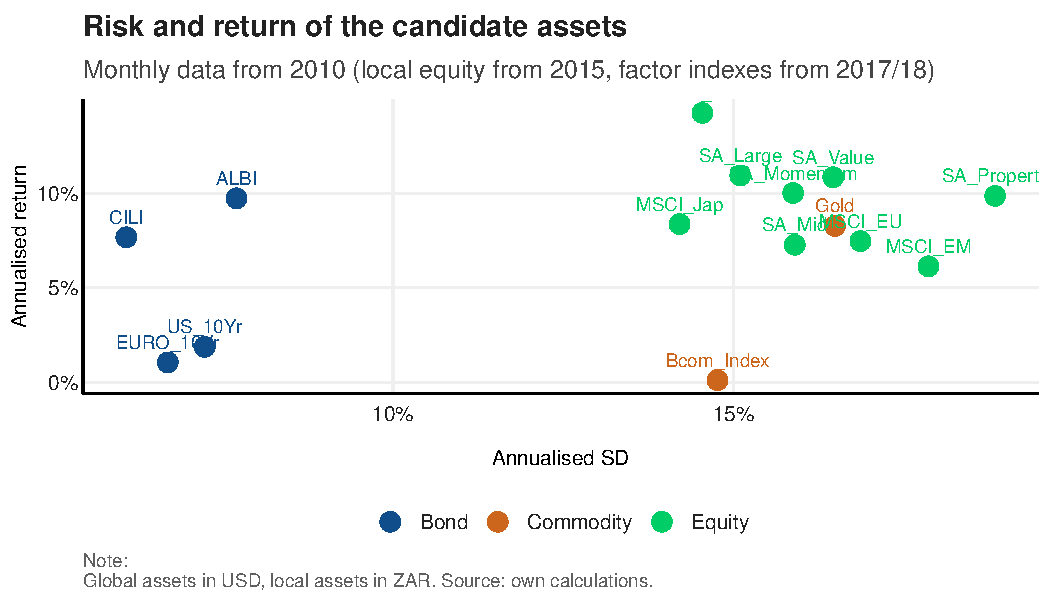
\includegraphics[keepaspectratio,alt={Risk and return of the candidate assets }]{Question4_files/figure-latex/Figure1-1.pdf}}
\caption{Risk and return of the candidate assets \label{Figure1}}
\end{figure}

The correlations (Figure \ref{Figure2}) shape what the optimiser can do.

\begin{itemize}
\tightlist
\item
  \textbf{Local bonds are not equity diversifiers.} The ALBI correlates
  0.52--0.66 with equities, because the rand drives both.
\item
  \textbf{Global bonds are the true diversifiers}, with correlations of
  only 0.0--0.35 with equities.
\item
  \textbf{The local equity indexes are close to one asset:} SA Large,
  Momentum and Value correlate 0.90--0.93.
\end{itemize}

\begin{figure}
\centering
\pandocbounded{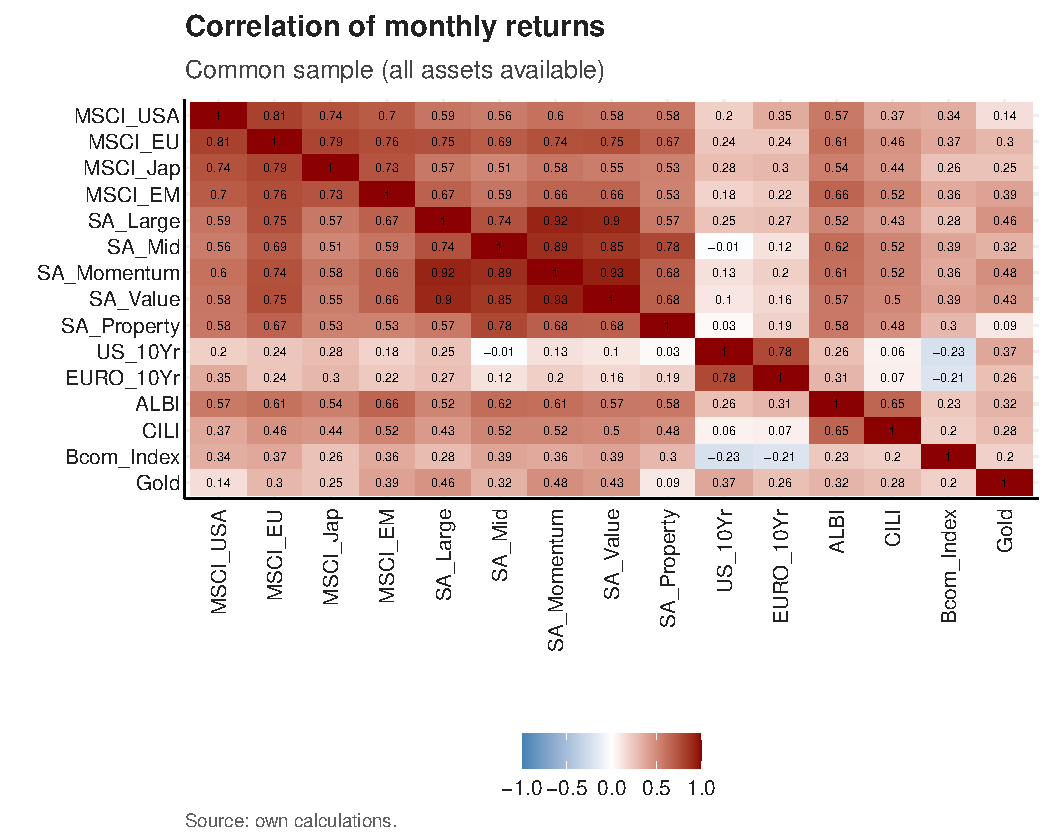
\includegraphics[keepaspectratio,alt={Correlation of monthly returns }]{Question4_files/figure-latex/Figure2-1.pdf}}
\caption{Correlation of monthly returns \label{Figure2}}
\end{figure}

\section{\texorpdfstring{Methodology
\label{Method}}{Methodology }}\label{methodology}

\subsection{Bond total-return proxy}\label{bond-total-return-proxy}

At each month-end \(t-1\), a 10-year par bond is bought with coupon
equal to the yield \(y_{t-1}\). At \(t\) it is re-priced at the new
yield, and one month of coupon is added. With semi-annual coupons, the
price of a bond with coupon \(c\) at yield \(y\) is

\[
P(y; c) = \sum_{k=1}^{20} \frac{c/2}{(1+y/2)^k} + \frac{1}{(1+y/2)^{20}},
\qquad
r_t = P(y_t; y_{t-1}) - 1 + \frac{y_{t-1}}{12}.
\]

Re-pricing the bond captures both duration and convexity, and remains
valid for negative yields.

\subsection{Expected returns and
covariance}\label{expected-returns-and-covariance}

Following the course's portfolio-optimisation practical, expected
returns are geometric means, the return each asset actually compounded
at:

\[
\hat{\mu}_i = \Big(\prod_{t=1}^{T}(1+R_{i,t})\Big)^{1/T} - 1.
\]

The sample covariance matrix is shrunk towards a structured target to
reduce estimation error
(\citeproc{ref-ledoit2003}{\textbf{ledoit2003?}};
\citeproc{ref-ledoit2004}{\textbf{ledoit2004?}}):

\[
\hat{\Sigma}_{LW} = (1-\rho)\,\hat{\Sigma} + \rho\, F,
\]

where \(\rho\) is the estimated optimal shrinkage intensity.
\(\hat{\Sigma}_{LW}\) is computed with the \texttt{covEstimation}
function of the \texttt{RiskPortfolios} package (type ``lw'') and made
positive definite with \texttt{nearPD} from the \texttt{Matrix} package.

\subsection{Missing returns}\label{missing-returns}

Assets that start after 2010 have gaps at the start of the estimation
window. As the course practical recommends, gaps are never set to zero,
since zero is a valid return and would bias the covariance. Instead,
each gap is filled with a random draw from the asset's own kernel
density \(\hat{f}_i\), which preserves its volatility. A fixed seed
makes this reproducible.

The practical's function uses the first asset's density probabilities
for every asset; here each asset uses its own density.

\subsection{Optimisation with the mandate's
constraints}\label{optimisation-with-the-mandates-constraints}

Let \(w\) be the vector of weights, and let \(\mathbb{1}_E\),
\(\mathbb{1}_B\), \(\mathbb{1}_C\) and \(\mathbb{1}_G\) indicate equity,
bond, commodity and global assets. The feasible set is

\[
\mathcal{C} = \Big\{ w : \mathbf{1}'w = 1,\;\; 0 \le w_i \le 0.35,\;\; \mathbb{1}_E'w \le 0.75,\;\; \mathbb{1}_B'w \le 0.25,\;\; \mathbb{1}_C'w \le 0.15,\;\; \mathbb{1}_G'w \le 0.60 \Big\}.
\]

\textbf{Minimum variance:}

\[
w^{MV} = \arg\min_{w \in \mathcal{C}} \; w'\hat{\Sigma}_{LW}\, w.
\]

\textbf{Maximum Sharpe ratio}
(\citeproc{ref-markowitz1952}{\textbf{markowitz1952?}}): maximising
\(w'\hat{\mu} / \sqrt{w'\hat{\Sigma}w}\) is not a quadratic programme.
Following the course practical, it is rewritten in scaled weights
\(\hat{w}\):

\[
\min_{\hat{w}} \; \hat{w}'\hat{\Sigma}_{LW}\,\hat{w}
\quad \text{s.t.} \quad
\hat{\mu}'\hat{w} = 1,\;\; \hat{w} \ge 0,\;\;
\hat{w}_i \le 0.35\,\mathbf{1}'\hat{w},\;\;
\mathbb{1}_g'\hat{w} \le \text{cap}_g\,\mathbf{1}'\hat{w},
\]

and then \(w = \hat{w}/\mathbf{1}'\hat{w}\). The caps must be written in
scaled form, because \(\hat{w}\) does not sum to one.

Both problems are solved with \texttt{quadprog::solve.QP}, which
minimises \(\tfrac{1}{2}w'Dw - d'w\) subject to \(A'w \ge b\). Upper
bounds enter as \(-w \ge -\text{cap}\).

\texttt{RiskPortfolios::optimalPortfolio}, used in the bonus practical,
accepts only per-asset bounds. It cannot impose the group caps, which is
why the constraint-matrix approach is needed.

\subsection{Rolling estimation and
rebalancing}\label{rolling-estimation-and-rebalancing}

At each quarter-end \(\tau\) from December 2019 to June 2026:

\begin{itemize}
\tightlist
\item
  An expanding window of monthly data from January 2010 to \(\tau\) is
  used, so every estimate uses at least 120 months.
\item
  Only assets with at least 60 months of actual returns are eligible.
\item
  Weights are computed for both optimisers. If an optimiser fails, the
  rules-based portfolio is used instead, as in the bonus practical's
  safe optimiser.
\end{itemize}

Weights decided at \(\tau\) are applied from month \(\tau+1\), and then
drift with prices until the next rebalance:

\[
R_{p,t} = \sum_i w^{BOP}_{i,t}\, R_{i,t}.
\]

This timing matters. \texttt{Safe\_Return.portfolio} with
\texttt{lag\_weights\ =\ TRUE} applies weights dated \(t\) to month
\(t\)'s return. Dating weights at the decision month would therefore let
each portfolio earn a return that was already in its estimation window,
a look-ahead bias. Weights are therefore dated at the first month they
are held.

\subsection{Benchmark, turnover and
drift}\label{benchmark-turnover-and-drift}

The \textbf{rules-based portfolio} holds fixed buckets, with equal
weights within each bucket:

\begin{itemize}
\tightlist
\item
  30\% global equity;
\item
  30\% local equity;
\item
  12.5\% local bonds;
\item
  12.5\% global bonds;
\item
  15\% commodities.
\end{itemize}

This puts 57.5\% offshore, within the 60\% cap.

\textbf{Turnover} at each rebalance is

\[
TO_\tau = \tfrac{1}{2}\sum_i \big|w^{\text{target}}_{i,\tau} - w^{\text{drift}}_{i,\tau}\big|.
\]

Drifted weights are checked against the caps every month.

\section{\texorpdfstring{Results
\label{Results}}{Results }}\label{results}

\subsection{Optimised weights and binding
constraints}\label{optimised-weights-and-binding-constraints}

Both optimisers converged at all 27 quarterly rebalances (December 2019
to June 2026), and every portfolio satisfies every constraint at every
rebalance (Table \ref{tab:checks}).

\begin{table}[!htbp]
\centering
\caption{Constraint checks at every rebalance (weights sum to 1; long only; single asset, equity, bond, commodity and global caps of 35\%, 75\%, 25\%, 15\% and 60\%)} 
\label{tab:checks}
\begingroup\scriptsize
\begin{tabular}{lrlllllll}
  \hline
Portfolio & Rebalances & Sum 1 & Long only & Single & Equity & Bonds & Commod. & Global \\ 
  \hline
MaxSharpe & 27 & Yes & Yes & Yes & Yes & Yes & Yes & Yes \\ 
  MinVol & 27 & Yes & Yes & Yes & Yes & Yes & Yes & Yes \\ 
  Static\_Balanced & 27 & Yes & Yes & Yes & Yes & Yes & Yes & Yes \\ 
   \hline
\end{tabular}
\endgroup
\end{table}

Table \ref{tab:exposure} shows which constraints bind.

\begin{itemize}
\tightlist
\item
  \textbf{The bond and commodity caps force equity to at least 60\%.}
  Bonds (\(\le 25\%\)) and commodities (\(\le 15\%\)) leave at least
  60\% for equity, so the 75\% equity cap never binds.
\item
  \textbf{The minimum-variance portfolio fills the bond cap and the 60\%
  global cap.} Global bonds and Japanese equity are its main low-risk
  building blocks.
\item
  \textbf{The maximum-Sharpe portfolio concentrates on the assets with
  the best past returns.} MSCI USA reaches the 35\% single-asset cap,
  alongside local inflation-linked bonds, gold and, later, the Value
  index.
\end{itemize}

\begin{table}[!htbp]
\centering
\caption{Average exposures across rebalances} 
\label{tab:exposure}
\begingroup\footnotesize
\begin{tabular}{lrrrrr}
  \hline
Portfolio & Equity & Bonds & Commodities & Global & Largest single asset \\ 
  \hline
MaxSharpe & 0.627 & 0.250 & 0.123 & 0.517 & 0.342 \\ 
  MinVol & 0.601 & 0.250 & 0.149 & 0.600 & 0.224 \\ 
  Static\_Balanced & 0.600 & 0.250 & 0.150 & 0.575 & 0.083 \\ 
   \hline
\end{tabular}
\endgroup
\end{table}

Figure \ref{Figure3} shows that the maximum-Sharpe weights swing much
more from quarter to quarter than the minimum-variance weights. This
instability is typical of optimisers that rely on estimated mean
returns, which are measured far less precisely than covariances. Table
\ref{tab:latest} gives the latest weights.

\begin{figure}
\centering
\pandocbounded{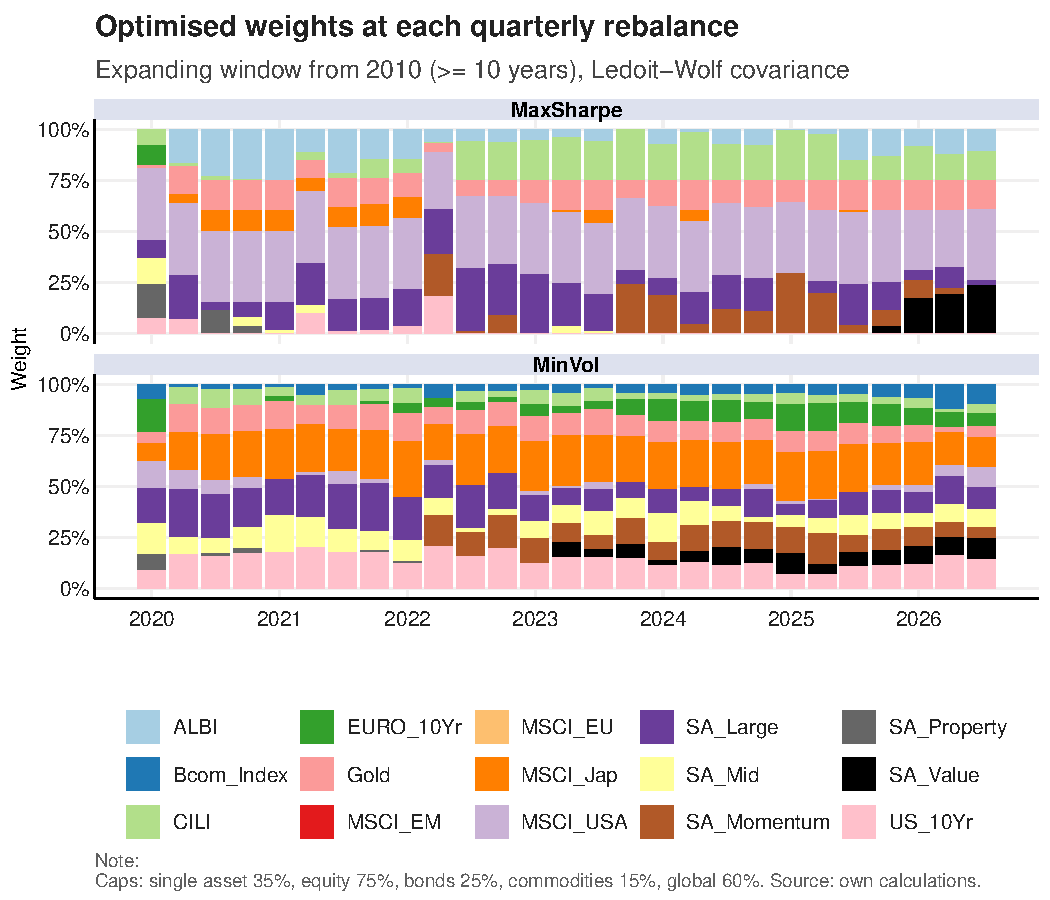
\includegraphics[keepaspectratio,alt={Optimised weights at each quarterly rebalance }]{Question4_files/figure-latex/Figure3-1.pdf}}
\caption{Optimised weights at each quarterly rebalance \label{Figure3}}
\end{figure}

\begin{table}[!htbp]
\centering
\caption{Weights at the latest rebalance (June 2026)} 
\label{tab:latest}
\begingroup\scriptsize
\begin{tabular}{lllrrr}
  \hline
Asset & Class & Region & MinVol & MaxSharpe & Static\_Balanced \\ 
  \hline
MSCI\_USA & Equity & Global & 0.098 & 0.350 & 0.075 \\ 
  MSCI\_EU & Equity & Global & 0.000 & 0.000 & 0.075 \\ 
  MSCI\_Jap & Equity & Global & 0.149 & 0.000 & 0.075 \\ 
  MSCI\_EM & Equity & Global & 0.000 & 0.000 & 0.075 \\ 
  SA\_Large & Equity & Local & 0.109 & 0.024 & 0.060 \\ 
  SA\_Mid & Equity & Local & 0.084 & 0.000 & 0.060 \\ 
  SA\_Momentum & Equity & Local & 0.057 & 0.000 & 0.060 \\ 
  SA\_Value & Equity & Local & 0.103 & 0.235 & 0.060 \\ 
  SA\_Property & Equity & Local & 0.000 & 0.000 & 0.060 \\ 
  US\_10Yr & Bond & Global & 0.142 & 0.000 & 0.062 \\ 
  EURO\_10Yr & Bond & Global & 0.062 & 0.000 & 0.062 \\ 
  ALBI & Bond & Local & 0.000 & 0.108 & 0.062 \\ 
  CILI & Bond & Local & 0.046 & 0.142 & 0.062 \\ 
  Bcom\_Index & Commodity & Global & 0.097 & 0.000 & 0.075 \\ 
  Gold & Commodity & Global & 0.053 & 0.141 & 0.075 \\ 
   \hline
\end{tabular}
\endgroup
\end{table}

\subsection{Out-of-sample performance}\label{out-of-sample-performance}

Table \ref{tab:stats} and Figure \ref{Figure4} compare the three
portfolios out of sample, from January 2020 to September 2026.

\begin{itemize}
\tightlist
\item
  \textbf{The optimisers do not clearly beat the simple rules-based
  portfolio.}

  \begin{itemize}
  \tightlist
  \item
    The \textbf{minimum-variance} portfolio delivered the smallest
    drawdown (16.4\%) and the smallest tail loss, but its volatility was
    barely lower (11.2\% against 11.4\%) and it returned 1.3\% a year
    less.
  \item
    The \textbf{maximum-Sharpe} portfolio earned about 1.2\% a year more
    than the rules-based portfolio, at the cost of a larger drawdown
    (20.5\%).
  \end{itemize}
\item
  \textbf{This echoes a well-known finding:} optimisers built on
  estimated inputs often struggle to beat simple diversified rules out
  of sample (\citeproc{ref-demiguel2009}{\textbf{demiguel2009?}}).
\end{itemize}

\begin{table}[!htbp]
\centering
\caption{Out-of-sample performance, Jan 2020 to Sep 2026 (monthly returns)} 
\label{tab:stats}
\begingroup\footnotesize
\begin{tabular}{lrrr}
  \hline
Info & MinVol & MaxSharpe & Static\_Balanced \\ 
  \hline
Cumulative return & 0.770 & 1.065 & 0.910 \\ 
  Return (ann.) & 0.088 & 0.113 & 0.101 \\ 
  SD (ann.) & 0.112 & 0.125 & 0.114 \\ 
  Return / risk & 0.811 & 0.924 & 0.902 \\ 
  Adj. Sharpe ratio & 0.706 & 0.680 & 0.705 \\ 
  Max drawdown & 0.164 & 0.205 & 0.180 \\ 
  Pain index & 0.027 & 0.027 & 0.026 \\ 
  Tracking error vs Static & 0.025 & 0.031 & 0.000 \\ 
  Modified CVaR (95\%, monthly) & -0.076 & -0.098 & -0.082 \\ 
   \hline
\end{tabular}
\endgroup
\end{table}

\begin{figure}
\centering
\pandocbounded{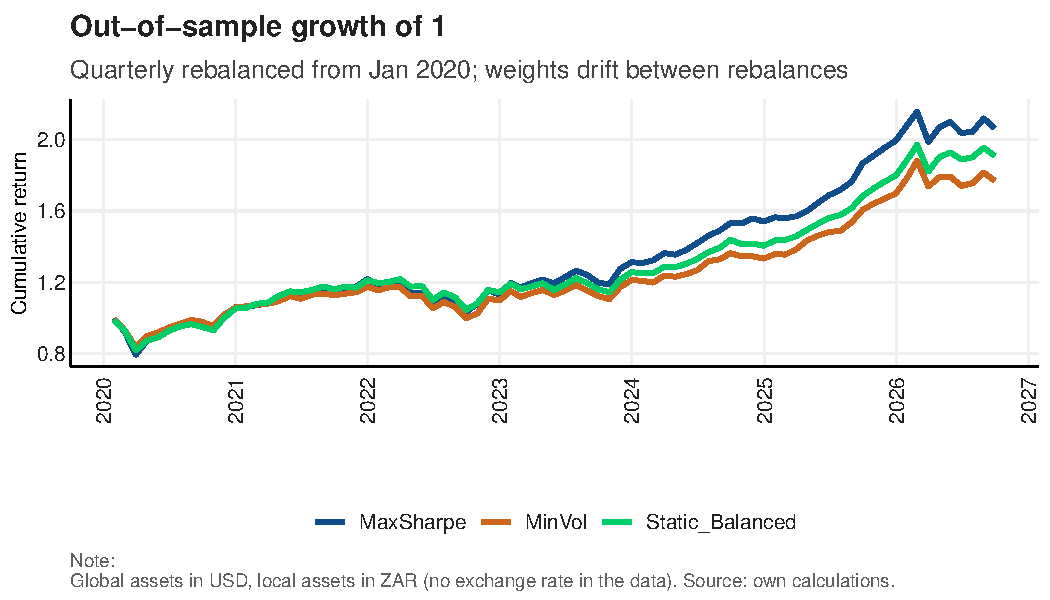
\includegraphics[keepaspectratio,alt={Out-of-sample growth of 1 }]{Question4_files/figure-latex/Figure4-1.pdf}}
\caption{Out-of-sample growth of 1 \label{Figure4}}
\end{figure}

A first version of the backtest gave much better results for the
optimisers. For example, the minimum-variance portfolio's volatility was
10.4\% and the maximum-Sharpe return 12.8\% a year. That version applied
each quarter's weights to the return of the month in which they were
estimated. Correcting this look-ahead bias (Section \ref{Method})
removed most of the optimisers' apparent advantage, which shows how
easily backtests can overstate the value of optimisation.

Calendar-year returns (Table \ref{tab:cal}) and drawdowns (Figure
\ref{Figure5}) show that \textbf{2022 was the hardest year for all three
portfolios (\(-6\%\) to \(-7\%\))}. Equities and bonds fell together, so
the bond allocation offered no protection. The maximum-Sharpe portfolio
led in the strong equity years of 2023--2024.

\begin{table}[!htbp]
\centering
\caption{Calendar-year returns} 
\label{tab:cal}
\begingroup\footnotesize
\begin{tabular}{lrrr}
  \hline
Year & MinVol & MaxSharpe & Static\_Balanced \\ 
  \hline
2020 & 0.060 & 0.060 & 0.053 \\ 
  2021 & 0.110 & 0.149 & 0.151 \\ 
  2022 & -0.066 & -0.071 & -0.056 \\ 
  2023 & 0.104 & 0.160 & 0.100 \\ 
  2024 & 0.099 & 0.174 & 0.117 \\ 
  2025 & 0.274 & 0.294 & 0.280 \\ 
  2026 (to Sep) & 0.042 & 0.035 & 0.062 \\ 
   \hline
\end{tabular}
\endgroup
\end{table}

\begin{figure}
\centering
\pandocbounded{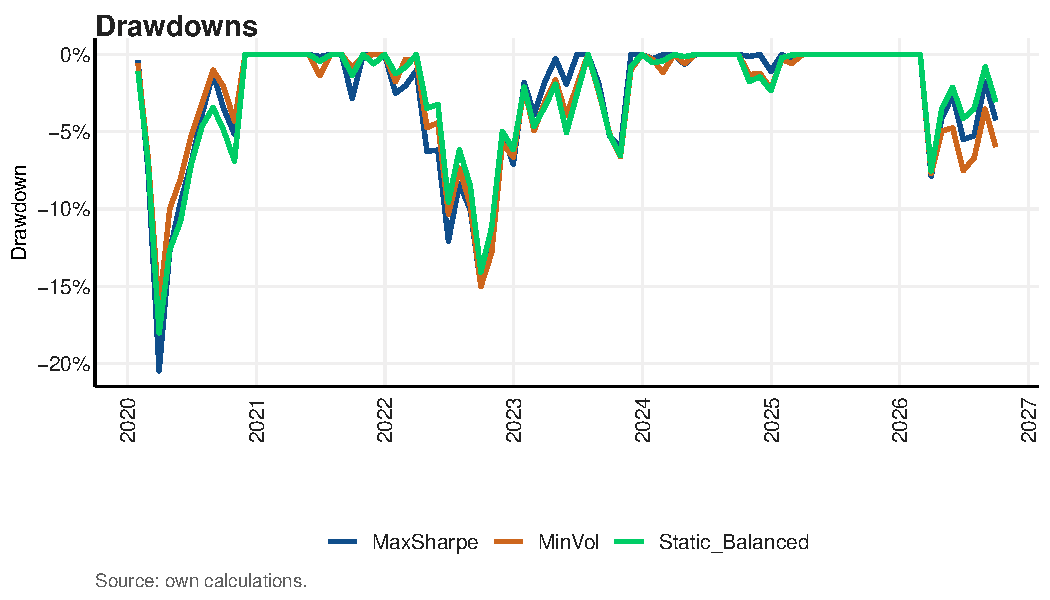
\includegraphics[keepaspectratio,alt={Drawdowns }]{Question4_files/figure-latex/Figure5-1.pdf}}
\caption{Drawdowns \label{Figure5}}
\end{figure}

\subsection{Turnover and drift}\label{turnover-and-drift}

Table \ref{tab:trade} reports implementation costs and drift.

\begin{itemize}
\tightlist
\item
  \textbf{The maximum-Sharpe portfolio trades about 70\% of the fund
  each year}, against 54\% for minimum variance and 11\% for the
  rules-based portfolio. Trading costs are not modelled, so they would
  narrow the maximum-Sharpe portfolio's return advantage.
\item
  \textbf{Drift pushes the portfolios past the caps between rebalances.}
  Because the optimisers sit at the bond, commodity and global limits,
  price moves take them over between rebalances, for example bonds up to
  28\% and global exposure up to 63\%.
\item
  \textbf{A practical fix} is to optimise to slightly tighter internal
  limits (for example the caps minus two percentage points), or to
  rebalance whenever a cap is breached.
\end{itemize}

\begin{table}[!htbp]
\centering
\caption{Annual turnover, number of months (of 81) in which drifted weights breach each cap, and the highest drifted bond and global weights} 
\label{tab:trade}
\begingroup\scriptsize
\begin{tabular}{lrrrrrrr}
  \hline
Portfolio & Turnover p.a. & Bonds & Commod. & Global & Single & Max bond & Max global \\ 
  \hline
MaxSharpe & 0.702 &   13 &   13 &    8 &   27 & 0.282 & 0.631 \\ 
  MinVol & 0.540 &    5 &   27 &   17 &    0 & 0.283 & 0.630 \\ 
  Static\_Balanced & 0.110 &   10 &   27 &    0 &    0 & 0.278 & 0.598 \\ 
   \hline
\end{tabular}
\endgroup
\end{table}

\section{\texorpdfstring{Model summary
\label{Summary}}{Model summary }}\label{model-summary}

\begin{table}[!htbp]
\centering
\caption{Summary of the three portfolios} 
\label{tab:summary}
\begingroup\scriptsize
\begin{tabular}{p{3.0cm}p{3.6cm}p{3.6cm}p{3.6cm}}
  \hline
  & Minimum variance & Maximum Sharpe & Rules-based \\ 
  \hline
Objective & Lowest variance & Best return per unit of risk & Fixed balanced buckets \\ 
  Inputs used & Covariance only & Means and covariance & None \\ 
  Binding constraints & Bonds 25\%, global 60\%, commodities & Bonds 25\%, single asset 35\% & Within all caps by design \\ 
  Weight stability & Fairly stable & Unstable & Fixed \\ 
  Out-of-sample return / risk & 8.8\% / 11.2\% & 11.3\% / 12.5\% & 10.1\% / 11.4\% \\ 
  Drawdown and tail risk & Smallest (16.4\%) & Largest (20.5\%) & Middle (18.0\%) \\ 
  Turnover & About 54\% a year & About 70\% a year & About 11\% a year \\ 
  Verdict & Recommended core strategy & Too reliant on noisy return forecasts & Strong, cheap benchmark \\ 
   \hline
\end{tabular}
\endgroup
\end{table}

Table \ref{tab:summary} summarises the three portfolios. All satisfy the
mandate at every rebalance. In practice, the bond and commodity caps
(which force at least 60\% into equity) and the 60\% global cap shape
the portfolios more than the equity cap does.

\textbf{The minimum-variance portfolio is recommended for a balanced
index fund.} It does not depend on return forecasts, its weights are
relatively stable, and it delivered the smallest drawdown and tail loss.

\begin{itemize}
\tightlist
\item
  \textbf{The rules-based portfolio} is a strong, low-cost alternative
  and a useful benchmark.
\item
  \textbf{The maximum-Sharpe portfolio} earned more, but its advantage
  rests on noisy estimates of expected returns, larger drawdowns and
  much higher turnover.
\end{itemize}

The main limitations are:

\begin{itemize}
\tightlist
\item
  the mix of currencies (US dollar global assets and rand local assets),
  with no exchange rate available;
\item
  the bond index proxies constructed from yields;
\item
  trading costs that are not modelled;
\item
  weight drift beyond the caps between quarterly rebalances;
\item
  the multi-asset file mentioned in the paper, which was not provided.
\end{itemize}

\newpage

\section*{References}\label{references}
\addcontentsline{toc}{section}{References}

\protect\phantomsection\label{refs}

\bibliography{Tex/ref}





\end{document}
